\documentclass{standalone}
\usepackage{pgfplots}
\pgfplotsset{compat=1.16}
\begin{document}
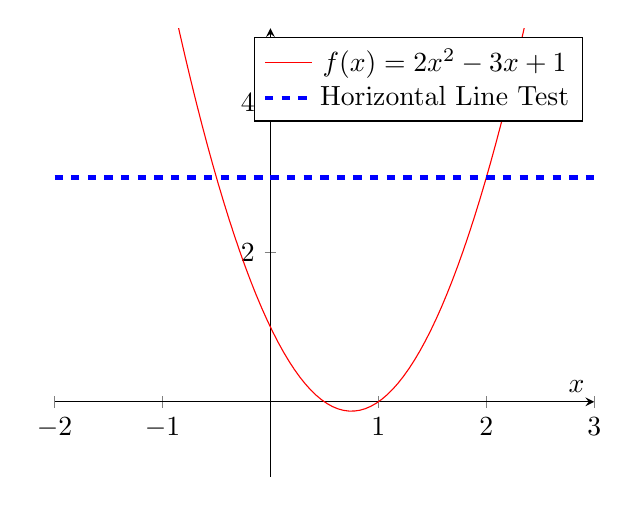
\begin{tikzpicture}
\begin{axis}[
    axis lines = middle,
    xlabel = $x$,
    ylabel = {$f(x)$},
    xmin=-2, xmax=3,
    ymin=-1, ymax=5
]
\addplot [
    domain=-2:3, 
    samples=100, 
    color=red,
]
{2*x^2-3*x+1};
\addplot [
    domain=-2:3, 
    samples=100, 
    color=blue,
    dashed,
    ultra thick
]
{3};
\legend{$f(x)=2x^2-3x+1$, Horizontal Line Test}
\end{axis}
\end{tikzpicture}
\end{document}
